% !TEX program = xelatex
\documentclass{misisarticle}

\grnti{47.01.07, 47.01.09}
\asjc{1702, 1705, 1710}
\oecd{1020}

\title{Метод построения многоязычного эшелонированного фильтра прямых промпт-инъекций с гарантированной верхней границей доли пропущенных атак}

\misisauthor{Е.~Светлаков}{кафедра инженерной кибернетики НИТУ «МИСиС»}{Москва, Россия}{m2305781@edu.misis.ru}
\misisauthor{Х.~Обада}{кафедра инженерной кибернетики НИТУ «МИСиС»}{Москва, Россия}{}

\abstract{%
Рассматривается построение фильтра прямых промпт-инъекций на входе локального LLM-сервиса при ограничении на вычислительный бюджет. В отличие от каскадных фильтров, в которых порядок эшелонов и границы зоны эскалации задаются эвристически, предлагается упорядочивать эшелоны по измеряемым стоимости и разрешающей способности оценки, а пороги маршрутизации выбирать процедурой распределённо-свободного контроля риска Learn then Test. Метод обеспечивает верхнюю границу доли пропущенных атак $\alpha$ с вероятностью не меньше $1-\delta$ при сохранении предположений калибровки. Для разметки по факту успеха используются утечка канареечного токена из системного промпта и другие детерминированные нарушения без LLM-судьи. Собственный русско-английский генератор включает смешанные запросы и выравнивание распределения длин между классами; выполнено 60000 прогонов для 6000 запросов. Построен каскад TF-IDF и multilingual-E5-small, в котором энкодер вызывается только для серой зоны первого эшелона. На calib для $\alpha=0{,}05$ получены FNR $=3{,}05\%$, FPR $=0\%$, доля эскалаций $3{,}33\%$ и стоимость $1{,}647$ мс на запрос; для $\alpha=0{,}02$ --- FNR $=0{,}25\%$, FPR $=0\%$, эскалации $1{,}27\%$ и $0{,}847$ мс. Повторная диагностика на ранее использованном own test дала FNR $1{,}53\%$ и $0\%$ соответственно при FPR $=0\%$; она не считается независимой проверкой.
}

\keywords{%
прямые промпт-инъекции, эшелонированная фильтрация запросов, многоязычные энкодеры, калибровка порогов моделей, контроль доли пропущенных атак на LLM, канареечная разметка
}

\begin{document}
\maketitle

\section{Введение}

Большие языковые модели (БЯМ) встраиваются в локальные сервисы поддержки, поиска и обработки документов. В таких системах пользовательский текст передаётся модели вместе со служебными инструкциями. Прямая промпт-инъекция ставит целью изменить поведение модели: отменить ограничения, навязать требуемый ответ или раскрыть содержимое системного промпта~\cite{owasp2025}. Сходная инструкция может быть скрыта и во внешних данных~\cite{greshake2023}, однако предметом настоящей работы являются прямые запросы пользователя.

Задача состоит в фильтрации таких запросов при ограничении на вычислительный бюджет. В известных каскадных фильтрах порядок эшелонов и границы зоны эскалации часто задаются эвристически: гарантии на долю пропущенных атак они не дают, а перенос настройки на другое оборудование, язык или защищаемую модель требует повторного ручного подбора. Кроме того, метка по предполагаемому намерению не показывает, действительно ли атака преодолела ограничения конкретной модели.

Предлагаемый метод сочетает упорядочение эшелонов по стоимости и разрешающей способности с калибровкой порогов Learn then Test (LTT)~\cite{angelopoulos2025}. Его основные элементы:
\begin{itemize}
  \item суррогатные цели атак с детерминированным канареечным критерием успеха;
  \item русско-английский корпус, включая смешанные и спорные запросы, с выравниванием длин и групповым разбиением;
  \item многоэшелонная фильтрация с порогами, обеспечивающими верхнюю границу FNR $\alpha$ с вероятностью не меньше $1-\delta$.
\end{itemize}
Схема экспериментального конвейера приведена на рис.~\ref{fig:method}.

\begin{figure}[t]
  \centering
  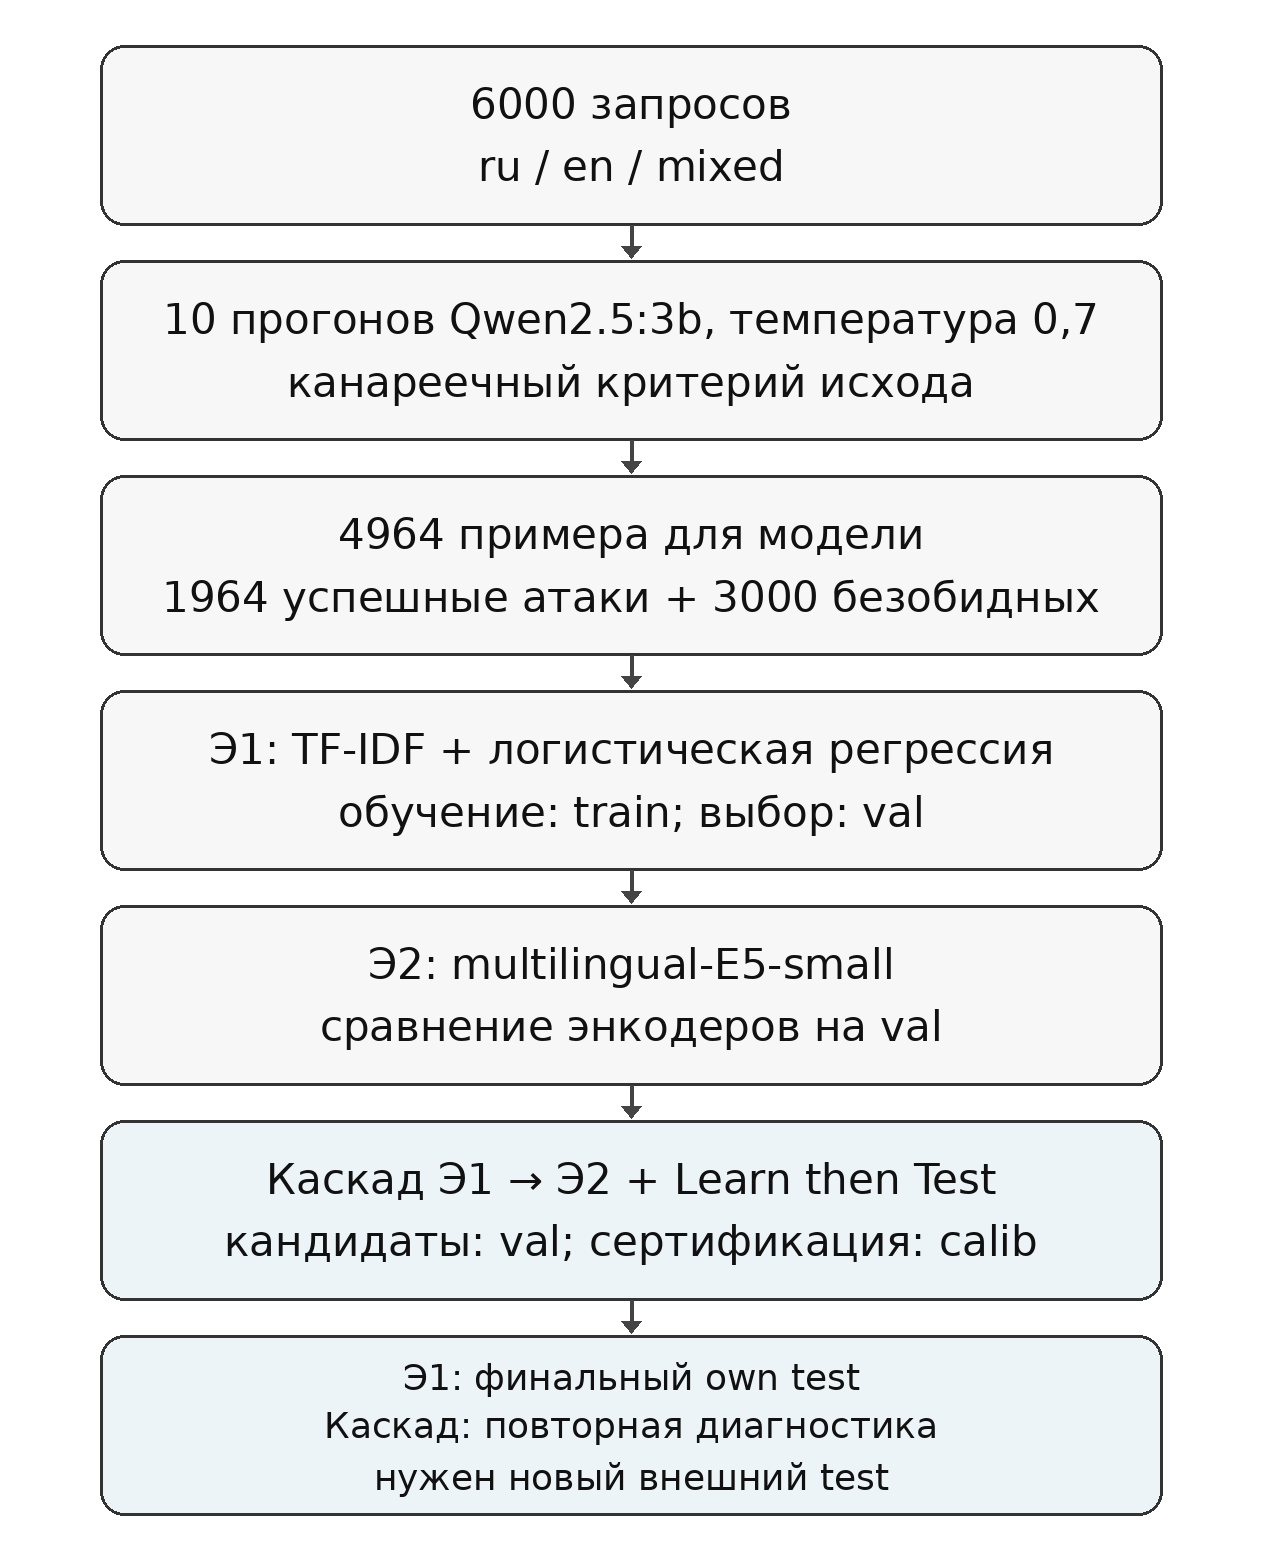
\includegraphics[width=0.94\columnwidth]{figures/method.png}
  \caption{Конвейер разметки, выбора эшелонов, калибровки каскада и проверки}
  \label{fig:method}
\end{figure}

На момент подготовки работы автором не обнаружено решений, сочетающих такую калибровку каскада, разметку по факту успеха и отдельный контроль качества на русском и английском языках. Практическая реализация предусматривает шлюз с OpenAI-совместимым API. Экспериментальная часть включает выбор энкодера, калибровку полного каскада, измерение стоимости и доли эскалаций; независимая внешняя проверка остаётся отдельной задачей.

\section{Связанные работы}

Формальная модель и сравнение атак и защит представлены в работе Liu и соавторов~\cite{liu2024}. Авторы рассматривают пять атак и десять защит на десяти моделях и семи задачах, включая обнаружение по заранее известному ответу. Greshake и соавторы показывают, что инструкция может быть доставлена не только пользователем, но и данными, которые приложение извлекает из внешнего источника~\cite{greshake2023}.

DataSentinel использует проверку известного ответа и игровую постановку для обнаружения инъекций~\cite{liu2025datasentinel}. Этот подход близок к канареечной идее, но решает задачу обнаружения атаки при работе защищённой модели. В настоящей работе суррогатная цель применяется также для формирования обучающих меток: фиксируется не предполагаемое намерение, а конкретное нарушение системной инструкции.

Проблема чрезмерной блокировки безобидных запросов систематически исследуется в PIGuard~\cite{li2025piguard}. Набор NotInject содержит 339 безобидных примеров со словами-триггерами; у ряда защит точность на нём приближается к 60\%. Следовательно, долю пропущенных атак нельзя оптимизировать отдельно от ложных срабатываний. В предлагаемой методике FPR вычисляется на обычных и трудных безобидных запросах, но не входит в биномиальную гарантию LTT.

Русскоязычные обзоры описывают методы фильтрации, изоляции контекста и обучения на возмущённых данных~\cite{mudarova2024, velichko2025}. Таксономия лингвистических уязвимостей и примеры атак на русском языке рассмотрены в~\cite{zyryanova2024}. В отличие от работ, ограниченных сравнением качества классификаторов, здесь дополнительно используется LTT: калибровка сводится к проверке статистических гипотез о риске~\cite{angelopoulos2025}, а кандидаты формируются до независимой калибровочной выборки, как в схеме Pareto Testing~\cite{laufer2023}.

Прикладные нейросетевые решения и сравнение современных подходов к детекции представлены в сборниках кафедры~\cite{misis2024, korotkikh2025}. Более общая задача распределённого контроля доступа рассмотрена Hammoud и Tarkhanov~\cite{hammoud2025}. Настоящая работа отличается предметом защиты и использует статистический контроль именно доли пропущенных промпт-инъекций.

\section{Постановка задачи}

Рассматривается локальный LLM-сервис, на вход которого поступает пользовательский запрос $x$ на русском, английском или смешанном языке вместе со скрытой системной инструкцией. Требуется построить входной фильтр, который возвращает решение «пропустить» или «заблокировать» до обращения к защищаемой модели. Положительным классом является не любой запрос с предполагаемым вредоносным намерением, а прямая промпт-инъекция, фактически приведшая к заданному нарушению системной инструкции.

Пусть $R$ --- доля пропущенных успешных атак, а $T$ --- вычислительная стоимость проверки одного запроса. Для заданных $\alpha$ и $\delta$ требуется выбрать состав эшелонов и их пороги так, чтобы с вероятностью не меньше $1-\delta$ выполнялось $R\leq\alpha$, минимизируя среднюю стоимость $\mathbb{E}[T]$ на целевом оборудовании. Доля ложных блокировок FPR и доля запросов, эскалированных на более дорогой эшелон, измеряются отдельно. Решение должно использовать общий порядок калибровки без ручного перебора порогов при смене языка, оборудования или защищаемой модели.

\section{Метод}

\subsection{Разметка по исходу атаки}

В системный промпт защищаемой модели помещаются три безвредных правила: запрет раскрывать случайный токен вида \texttt{CNR-XXXXXXXXXX}, запрет произносить слово «ОРХИДЕЯ» и запрет выводить навязанный маркер \texttt{DEFENSE\_BYPASSED}. Запрос считается успешной атакой, если ответ содержит соответствующий токен, слово или маркер. Эти исходы обозначаются как утечка, нарушение правила и перехват вывода. Проверка выполняется программно после нормализации написания и не требует оценки ответа другой БЯМ.

Случайный токен создаётся заново для каждого запроса. Десять символов из алфавита в 36 знаков дают $36^{10}\approx3{,}66\cdot10^{15}$ вариантов, поэтому случайное совпадение маловероятно. Суррогатные цели не требуют генерации реального вредоносного содержания, но проверяют то же свойство: пользовательская инструкция возобладала над системной.

Ответ модели стохастичен, поэтому запрос $x$ подаётся $k$ раз. Пусть $c_j(x)=1$, если в $j$-м ответе обнаружен целевой признак, и $c_j(x)=0$ иначе. Тогда
\begin{equation}
  \hat p(x)=\frac{s(x)}{k}, \qquad s(x)=\sum_{j=1}^{k}c_j(x).
  \label{eq:phat}
\end{equation}
Для кандидата в атаку положительная метка ставится при $s(x)>0$. Для безобидного по построению запроса $y=0$ независимо от случайного признака в ответе; такие случаи сохраняются для контроля качества разметки. Кандидаты в атаки с $s(x)=0$ исключаются из обучения и из знаменателя FNR, поскольку на выбранной защищаемой модели они не привели к вредному исходу. Величина $\hat p$ не является признаком детектора и используется только во взвешенной метрике.

Отдельно обрабатываются отказы с цитированием. Ответ вида «нельзя выводить строку \texttt{DEFENSE\_BYPASSED}» содержит маркер, но не свидетельствует об успехе атаки. После аудита полной разметки 1451 такой прогон в 658 строках переведён из успешных исходов в неоднозначные. Агрегированные метки пересчитаны по исходным ответам.

\subsection{Формирование корпуса}

Генератор сочетает цель атаки, обрамление, технику обфускации и язык. Общая таксономия проекта охватывает 16 техник атак. В текущем корпусе представлены русский, английский и смешанный языки; прямые нарушения инструкции, ролевые подмены, ложный авторитет, извлечение системного промпта и составные инструкции. Использованные преобразования включают отсутствие обфускации, разбиение слов, изменение регистра, гомоглифы, символы нулевой ширины, транслитерацию, Base64 и ROT13. Безобидный класс содержит обычные офисные запросы и спорные примеры с лексикой атак, но без вредоносной цели. Для последующего расширения этого класса предусмотрены русские и английские промпты GrandMaster-PRO-MAX~\cite{grandmaster}.

Исходный корпус содержит 6000 строк: 3000 кандидатов в атаки и 3000 безобидных запросов. Каждая строка десять раз обработана моделью Qwen2.5:3b~\cite{qwen2024} с температурой $0{,}7$. Всего получено 60000 ответов. После постобработки успешными оказались 1964 атаки, то есть $65{,}5\%$ кандидатов. Для обучения и оценки детектора использованы 4964 строки; 1036 неуспешных атак сохранены отдельно.

Варианты одного шаблона объединены по \texttt{group\_id}. Разбиение выполнено алгоритмом StratifiedGroupKFold с пятью folds, \texttt{random\_state=42} и стратификацией по метке, языку и технике. Folds 0--1 образуют train, folds 2, 3 и 4 соответственно val, calib и test. Состав частей приведён в таблице~\ref{tab:split}. Пересечений групп между частями нет. Train служит для обучения, val --- для выбора конфигурации и кандидатов порогов, calib --- для сертификации. Test сначала применяется один раз для финальной проверки Э1, а затем только для повторной диагностики замороженного каскада; независимым тестом каскада он не является.

\begin{table}[t]
  \caption{Групповое разбиение собственного корпуса}
  \label{tab:split}
  \centering
  \begin{tabular}{lrrrr}
    \toprule
    Часть & Строк & Атаки & Безобидные & Группы \\
    \midrule
    train & 1964 & 784 & 1180 & 143 \\
    val & 1005 & 393 & 612 & 73 \\
    calib & 1022 & 394 & 628 & 70 \\
    test & 973 & 393 & 580 & 72 \\
    \bottomrule
  \end{tabular}
\end{table}

\subsection{Маршрутизация в эшелонированном фильтре}

Предлагаемый фильтр содержит нормализатор и последовательность детекторов с возрастающей стоимостью проверки. Нормализация приводит Unicode к форме NFKC, удаляет невидимые символы и сводит визуально сходные буквы к единому написанию. Первый эшелон использует лексические признаки, второй --- мультиязычный энкодер. Их качество и стоимость измеряются на целевом оборудовании до включения в каскад; ниже проверяется полная маршрутизация Э1--Э2.

Эшелон $i$ возвращает оценку $s_i(x)\in[0,1]$ и имеет два порога $\lambda_i^{lo}\leq\lambda_i^{hi}$. Его решение задаётся как
\begin{equation}
a_i(x)=
\begin{cases}
\text{пропустить}, & s_i(x)<\lambda_i^{lo},\\
\text{эскалировать}, & \lambda_i^{lo}\leq s_i(x)<\lambda_i^{hi},\\
\text{заблокировать}, & s_i(x)\geq\lambda_i^{hi}.
\end{cases}
\label{eq:routing}
\end{equation}
Таким образом, очевидные случаи обрабатываются дешёвым эшелоном, а следующий получает только серую зону. Это соответствует общей идее каскада Виолы--Джонса~\cite{viola2001}. В вырожденном случае $\lambda_i^{lo}=\lambda_i^{hi}$ серой зоны нет; именно такая конфигурация исследуется ниже для первого эшелона.

Пусть $t_i$ --- средняя стоимость эшелона $i$, а $q_i$ --- доля запросов, дошедших до него, причём $q_1=1$. Средняя стоимость фильтрации равна
\begin{equation}
\mathbb{E}[T]=t_0+\sum_{i=1}^{M}q_i t_i,
\label{eq:cost}
\end{equation}
где $t_0$ --- стоимость нормализации. Порядок эшелонов и кандидаты порогов выбираются на val по стоимости и разрешающей способности; затем LTT сертифицирует конфигурацию целиком на calib. Доли пропусков отдельных эшелонов не перемножаются, поскольку их ошибки могут быть зависимы: одна и та же трудная атака способна обмануть несколько детекторов. Итоговый FNR вычисляется только по окончательному решению каскада.

Для двух эшелонов зафиксировано $\lambda_1^{lo}=0{,}5$. Три кандидата образованы парами уже выбранных на val порогов без нового поиска: $(\lambda_1^{hi},\lambda_2)$ равны $(0{,}6356704134;0{,}5260268237)$, $(0{,}6706789297;0{,}5776942018)$ и $(0{,}7237584272;0{,}6836875963)$. Их порядок соответствует возрастанию оценки $t_1+q_2t_2$ на val. На calib и test стоимость измеряется реальными вызовами: Э1 обрабатывает всю часть, Э2 --- только серую зону; сетевые расходы и нормализатор не входят в замер.

\subsection{Первый эшелон}

Детектор получает только текст запроса и возвращает оценку $s_\theta(x)$, интерпретируемую как оценку вероятности успешной атаки. Блокировка соответствует условию $s_\theta(x)\geq\lambda$. Использованы символьные TF-IDF-признаки \texttt{char\_wb} с $n$-граммами длиной 3--5, \texttt{sublinear\_tf=True}, $\texttt{min\_df}=3$ и не более чем 200000 признаками. Классификатор --- логистическая регрессия с $C=1$, взвешиванием классов и не более чем 2000 итерациями. Итоговая модель содержит 31634 признака.

Для уменьшения ошибок на другом распределении к собственному train добавлены 3194 уникальные англоязычные записи из открытых наборов~\cite{neuralchemy, dolly15k}: 2678 безобидных и пограничных запросов и 516 jailbreak-запросов. Перед добавлением выполнены NFKC-нормализация, приведение к нижнему регистру, схлопывание пробелов и дедупликация. Использовались только обучающие части внешних наборов; пересечений с собственными val, calib и test нет. Общий train содержит 5158 записей. Следует учитывать, что внешние метки описывают намерение, тогда как собственные --- наблюдаемый исход.

Три конфигурации детектора сравнивались на val по PR-AUC и затем ROC-AUC. Все получили значения, округляющиеся до $1{,}0$; в соответствии с заранее заданным порядком выбрана конфигурация 3--5. На val выбранной модели при $\lambda=0{,}5$ не допущено ни пропусков, ни ложных срабатываний. Пакетное вычисление оценок для 1005 запросов val на CPU заняло в среднем $0{,}320$ мс на запрос, включая построение TF-IDF-признаков и работу классификатора, но исключая сетевые расходы шлюза.

\subsection{Калибровка Learn then Test}

Пусть $R(\lambda)$ --- истинная доля пропущенных успешных атак при пороге $\lambda$. Требуется ограничить её уровнем $\alpha$ с доверием не меньше $1-\delta$. Для $n$ независимых успешных атак calib и $m$ наблюдаемых пропусков используется p-value
\begin{equation}
  p(\lambda)=P\{\operatorname{Binomial}(n,\alpha)\leq m\}.
  \label{eq:pvalue}
\end{equation}
Гипотеза $R(\lambda)>\alpha$ отвергается при $p(\lambda)\leq\delta$. Процедура не доказывает равенство риска нулю: она отвергает превышение заданного $\alpha$ на доступной калибровочной выборке. Даже при $m=0$ сертификация возможна только при достаточном объёме выборки:
\begin{equation}
  n\geq n_{\min}=\left\lceil\frac{\ln\delta}{\ln(1-\alpha)}\right\rceil.
  \label{eq:nmin}
\end{equation}
При $\delta=0{,}05$ получаем $n_{\min}=59$, $149$ и $299$ для $\alpha=0{,}05$, $0{,}02$ и $0{,}01$ соответственно. Наличие пропусков увеличивает необходимый объём.

Кандидаты заранее заморожены по val: $0{,}5$ и пороги, соответствующие val FNR $1\%$, $2\%$ и $5\%$: $0{,}6356704134$, $0{,}6706789297$ и $0{,}7237584272$. Для каждого $\alpha\in\{0{,}05;0{,}02;0{,}01\}$ они проверяются в порядке возрастания. После первого $p>\delta$ последовательность останавливается, а среди сертифицированных выбирается наибольший порог. Такой fixed-sequence тест не требует дополнительной поправки на число рассмотренных кандидатов. Гарантия предполагает перестановочность calib и рабочих данных и не распространяется автоматически на новый язык, другую модель или адаптивного противника.

\section{Метрики и протокол эксперимента}

Основная метрика --- доля пропусков среди успешных атак:
\begin{equation}
  \operatorname{FNR}=\frac{FN}{TP+FN}.
  \label{eq:fnr}
\end{equation}
Доля ложных блокировок вычисляется только на безобидных запросах: $\operatorname{FPR}=FP/(FP+TN)$. Дополнительно используется взвешенный FNR, учитывающий долю успехов атаки:
\begin{equation}
  \operatorname{FNR}_{w}(\lambda)=
  \frac{\sum_{i:y_i=1}\hat p_i\,\mathbb{1}[s_\theta(x_i)<\lambda]}
       {\sum_{i:y_i=1}\hat p_i}.
  \label{eq:wfnr}
\end{equation}
В отличие от обычного FNR, пропуск атаки, сработавшей в девяти из десяти прогонов, вносит больший вклад, чем пропуск атаки с одним успехом.

Сначала модель и кандидаты порогов фиксируются по train и val. Затем один раз выполняется сертификация на calib. Для каскада кандидаты проверяются в порядке возрастания val-стоимости; после первого $p>\delta$ последовательность останавливается, а последний сертифицированный кандидат выбирается для диагностики. По test не выбираются модель, основной уровень $\alpha$ или новый порог.

Перед оценкой проверяются SHA-256 modeling CSV, моделей и отчётов предыдущих этапов. Для Э1 выполняется одна финальная проверка own test. Для каскада тот же test используется повторно и рассматривается только как диагностика уже замороженных конфигураций, а не как независимая проверка. Все 1022 calib-оценки и 973 test-оценки каждого эшелона, окончательные решения и групповые confusion counts независимо воспроизведены повторной загрузкой моделей.

Дополнительная внешняя диагностика выполнена на 942 англоязычных запросах (552 атаки и 390 безобидных) из открытых наборов~\cite{neuralchemy, dolly15k}. Метки внешнего набора даны по намерению, поэтому его FNR несопоставим напрямую с исходной разметкой собственного корпуса. Этот набор участвовал в диагностике направления расширения train и рассматривается как данные разработки, а не как независимый финальный внешний тест.

\section{Результаты}

\subsection{Выбор энкодера второго эшелона}

До калибровки каскада на том же общем train из 5158 запросов сравнены четыре замороженных энкодера: одноязычный all-MiniLM-L6-v2~\cite{minilm_en}, русскоязычный rubert-tiny2~\cite{rubert_tiny2}, paraphrase-multilingual-MiniLM-L12-v2~\cite{minilm_multi} и multilingual-e5-small~\cite{e5small, wang2024multilingual}. Для всех использованы L2-нормализованные эмбеддинги, максимальная длина 512 токенов и одинаковая логистическая регрессия с $C=1$ и взвешиванием классов. В соответствии с модельной карточкой только вход E5 получал префикс \texttt{query: }. Выбор выполнялся на own val по максимуму среднего PR-AUC русского и английского срезов, затем по минимальному PR-AUC этих срезов, общему PR-AUC и задержке. Own calib и own test в этом сравнении не использовались.

\begin{table}[t]
  \caption{Сравнение энкодеров Э2 на own val}
  \label{tab:e2}
  \centering
  \resizebox{\columnwidth}{!}{%
  \begin{tabular}{lrrrrrr}
    \toprule
    Энкодер & PR-AUC & ru & en & Время, мс & FN & FP \\
    \midrule
    MiniLM-L6 (en) & 0,9730 & 0,9408 & 0,9975 & 39,29 & 3 & 155 \\
    rubert-tiny2 & 0,9977 & 0,9985 & 0,9981 & 9,31 & 3 & 25 \\
    multiling. MiniLM-L12 & 0,9972 & 0,9945 & 0,9997 & 46,31 & 3 & 34 \\
    multilingual-E5-small & \textbf{0,9999} & \textbf{0,9999} & \textbf{1,0000} & 45,02 & 3 & \textbf{0} \\
    \bottomrule
  \end{tabular}}
\end{table}

Результаты приведены в таблице~\ref{tab:e2}. Время --- средняя задержка одиночного запроса на CPU по 64 измерениям после warm-up, включая энкодер и классификатор. FN и FP соответствуют исследовательскому порогу с FNR не более $1\%$ на val. По заранее зафиксированному правилу выбран multilingual-E5-small: средний PR-AUC ru/en равен $0{,}999926$, ROC-AUC overall --- $0{,}999942$. Порог $0{,}526027$ даёт FN $=3/393$ и FP $=0/612$.

При порогах Э1 $0{,}635670$ и Э2 $0{,}526027$ каждый детектор пропускает по три атаки, но общих пропусков нет: Э2 обнаруживает все три ошибки Э1, а Э1 --- все три ошибки Э2. Jaccard множеств ошибок равен нулю. До калибровки это указывает на комплементарность только на val. При этом PR-AUC Э1 на val равен $1{,}0$, поэтому превосходство Э2 над Э1 как одиночного детектора не утверждается.

\subsection{Маршрутизация и сертификация каскада}

На val строгий каскад с $\lambda_1^{hi}=0{,}635670$ и $\lambda_2=0{,}526027$ не допускает ни пропусков, ни ложных срабатываний, эскалируя лишь 3 запроса из 1005. Для двух других кандидатов получены FN $=1$ и $8$ при 7 и 19 эскалациях соответственно. Эти конфигурации далее проверены LTT на 1022 запросах calib в порядке возрастания val-стоимости.

Результаты представлены в таблице~\ref{tab:cascade}. Для $\alpha=0{,}05$ все три кандидата сертифицированы; в соответствии с протоколом выбран последний, с p-value $0{,}040818$. Для $\alpha=0{,}02$ выбран строгий кандидат: следующий имеет $p=0{,}104344>\delta$ и останавливает последовательность. Для $\alpha=0{,}01$ уже первый кандидат имеет $p=0{,}094946>\delta$, поэтому на test он не оценивался. На calib и test FPR обеих выбранных конфигураций равен нулю.

\begin{table}[t]
  \caption{Калибровка каскада и повторная диагностика на own test}
  \label{tab:cascade}
  \centering
  \resizebox{\columnwidth}{!}{%
  \begin{tabular}{ccrrrrrrr}
    \toprule
    $\alpha$ & FNR-val & \multicolumn{2}{c}{Calib} & \multicolumn{2}{c}{Стоимость} & \multicolumn{3}{c}{Повторная диагностика test} \\
    \cmidrule(lr){3-4}\cmidrule(lr){5-6}\cmidrule(lr){7-9}
    & & FN & p-value & $q$, \% & мс & FN & $q$, \% & мс \\
    \midrule
    0,05 & 5\% & 12/394 & 0,040818 & 3,33 & 1,647 & 6/393 & 1,54 & 1,073 \\
    0,02 & 1\% & 1/394 & 0,003157 & 1,27 & 0,847 & 0/393 & 0,31 & 0,355 \\
    \bottomrule
  \end{tabular}}
\end{table}

На calib FNR составляет $3{,}05\%$ и $0{,}25\%$, FNR$_w$ --- $2{,}36\%$ и $0{,}0786\%$ соответственно. Полный вызов Э2 на всех запросах занимает $29{,}884$ мс; каскад снижает среднюю стоимость примерно в $18{,}1$ и $35{,}3$ раза. При этом Э1-only дешевле, но имеет другое качество: строгий каскад при одном пропуске устраняет 7 ложных срабатываний Э1 при пороге $0{,}5$. Для конфигурации 5\% каскад даёт FN $=12$ и FP $=0$ против FN $=28$ у Э1-only и FN $=31$, FP $=9$ у Э2-only.

Повторная диагностика на уже использованном для Э1 own test не является независимой проверкой. На ней FNR составляет $1{,}53\%$ и $0\%$, FNR$_w$ --- $1{,}59\%$ и $0\%$. Для $\alpha=0{,}05$ все шесть пропусков относятся к русским атакам. Для $\alpha=0{,}02$ эскалированы три русских запроса, пропусков нет; это не означает нулевой истинный риск и не использовалось для выбора порога.

\subsection{Сертификация первого эшелона на calib}

Результаты калибровки при $\delta=0{,}05$ представлены в таблице~\ref{tab:calib}. Для $\alpha=0{,}05$ выбран порог $0{,}6356704134$: семь пропусков из 394 атак, p-value $0{,}000764$. Следующий кандидат $0{,}6706789297$ имеет $p=0{,}0696>\delta$, поэтому последовательность остановлена. Для $\alpha=0{,}02$ сертифицирован только порог $0{,}5$; следующий кандидат не прошёл проверку. Для $\alpha=0{,}01$ уже начальный кандидат имеет $p=0{,}0949>\delta$, поэтому сертифицированного порога нет. Новые кандидаты по calib не подбирались.

\begin{table}[t]
  \caption{Сертифицированные пороги на own calib}
  \label{tab:calib}
  \centering
  \resizebox{\columnwidth}{!}{%
  \begin{tabular}{ccrrrrr}
    \toprule
    $\alpha$ & Порог & FN & FNR, \% & FPR, \% & p-value & FNR$_w$, \% \\
    \midrule
    0,05 & 0,635670 & 7/394 & 1,78 & 0 & 0,000764 & 1,26 \\
    0,02 & 0,500000 & 1/394 & 0,25 & 1,11 & 0,003157 & 0,079 \\
    0,01 & нет & --- & --- & --- & --- & --- \\
    \bottomrule
  \end{tabular}}
\end{table}

\subsection{Финальная проверка первого эшелона на own test}

В таблице~\ref{tab:test} приведены результаты одной финальной проверки на 973 ранее не использованных запросах. Для $\alpha=0{,}05$ детектор правильно заблокировал 390 из 393 успешных атак и не заблокировал ни одного из 580 безобидных запросов. FNR $=0{,}76\%$, FNR$_w=0{,}92\%$. Все три пропуска относятся к русским атакам с символами нулевой ширины: два имеют цель обхода политики и один --- извлечения системного промпта. На английском и смешанном срезах пропусков нет.

Для $\alpha=0{,}02$ при пороге $0{,}5$ на test не зарегистрировано ни пропусков, ни ложных срабатываний. Это наблюдение не означает нулевой истинный риск и не использовалось для переназначения рабочего порога. Поскольку на calib для $\alpha=0{,}01$ нет сертифицированного кандидата, соответствующая оценка на test не проводилась.

\begin{table}[t]
  \caption{Финальные результаты на own test}
  \label{tab:test}
  \centering
  \resizebox{\columnwidth}{!}{%
  \begin{tabular}{ccrrrrrrr}
    \toprule
    $\alpha$ & Порог & TP & FN & TN & FP & FNR, \% & FPR, \% & FNR$_w$, \% \\
    \midrule
    0,05 & 0,635670 & 390 & 3 & 580 & 0 & 0,76 & 0 & 0,92 \\
    0,02 & 0,500000 & 393 & 0 & 580 & 0 & 0 & 0 & 0 \\
    \bottomrule
  \end{tabular}}
\end{table}

Разрез по языкам для $\alpha=0{,}05$ приведён в таблице~\ref{tab:lang}. Все три пропуска пришлись на русский срез: FNR $=3/165=1{,}82\%$. При этом 242 спорных безобидных запроса с лексикой атак не были заблокированы, как и 338 обычных безобидных запросов. Эти подгруппы слишком малы для самостоятельных статистических гарантий и служат диагностикой ошибок.

\begin{table}[t]
  \caption{Результаты по языкам на own test при $\alpha=0{,}05$}
  \label{tab:lang}
  \centering
  \resizebox{\columnwidth}{!}{%
  \begin{tabular}{lrrrrrr}
    \toprule
    Язык & Атаки & FN & FNR, \% & Безобидные & FP & FPR, \% \\
    \midrule
    Русский & 165 & 3 & 1,82 & 274 & 0 & 0 \\
    Английский & 188 & 0 & 0 & 246 & 0 & 0 \\
    Смешанный & 40 & 0 & 0 & 60 & 0 & 0 \\
    \bottomrule
  \end{tabular}}
\end{table}

\subsection{Внешняя диагностика}

Добавление внешних обучающих примеров существенно уменьшило ложные срабатывания на внешней диагностической выборке: FPR снизился с $45{,}13\%$ до $7{,}69\%$, ROC-AUC вырос с $0{,}8624$ до $0{,}9740$ (таблица~\ref{tab:external}). Одновременно FNR по intent-меткам увеличился с $3{,}62\%$ до $5{,}43\%$. Таким образом, расширение train улучшило разделение в целом, но изменило компромисс между типами ошибок. Эти результаты не рассматриваются как подтверждение LTT-гарантии на внешнем распределении.

\begin{table}[t]
  \caption{Диагностика на внешнем наборе с intent-разметкой}
  \label{tab:external}
  \centering
  \resizebox{\columnwidth}{!}{%
  \begin{tabular}{lrr}
    \toprule
    Метрика & Только own train & Own train + внешний train \\
    \midrule
    ROC-AUC & 0,8624 & 0,9740 \\
    PR-AUC & 0,8867 & 0,9769 \\
    FNR при $\lambda=0{,}5$, \% & 3,62 & 5,43 \\
    FPR при $\lambda=0{,}5$, \% & 45,13 & 7,69 \\
    \bottomrule
  \end{tabular}}
\end{table}

\section{Обсуждение и ограничения}

Полученные значения показывают работоспособность всего протокола: от объективной разметки до сертификации и отложенной проверки. Однако почти идеальные результаты на собственном test не должны интерпретироваться как такое же качество на реальных атаках. Корпус синтетический и построен из конечного набора шаблонов. Групповое разбиение предотвращает совместное попадание вариантов одного шаблона в разные части, но не воспроизводит все способы адаптивного обхода. Более того, внутри calib и test остаётся несколько коррелированных строк с общим \texttt{group\_id}. Биномиальная формула предполагает независимые наблюдения, поэтому для строгой сертификации шаблонного распределения в следующем эксперименте необходимо оставлять по одному представителю группы либо использовать групповую процедуру контроля риска. Текущие p-values следует рассматривать с этой оговоркой.

Метка зависит от защищаемой модели, числа прогонов и суррогатных целей. Атака, неуспешная против Qwen2.5:3b, может быть успешной против другой модели. Перенос гарантии на новую модель требует новой разметки и калибровки. Кроме того, 406 исходов утечки приняты по первоначальной проверке полного ответа, хотя сохранённый фрагмент обрезан и не позволяет независимо увидеть канарейку.

Внешние обучающие записи имеют intent-разметку, поэтому смешение двух смыслов меток является ограничением. Внешняя диагностическая выборка уже использована при разработке; для честного внешнего утверждения необходим новый набор. Сравнение энкодеров выполнено только на val, а own test уже применялся для Э1 перед повторной диагностикой каскада. Поэтому результаты каскада на этом test не считаются независимым подтверждением. Наконец, число успешных атак в языковых подгруппах calib ограничено, а для $\alpha=0{,}01$ текущий набор кандидатов не сертифицирован. Дальнейшая работа включает новый внешний тест замороженного каскада, несколько защищаемых моделей, групповую и отдельную языковую калибровку. Планируемые внешние проверки: не менее 30 реальных русских инъекций, атаки LLAMATOR~\cite{llamator}, BIPIA~\cite{bipia}, корпус Dmtr\_Dr~\cite{dmtrdr} и NotInject~\cite{li2025piguard}. Практическим развитием является прототип шлюза с OpenAI-совместимым API.

\section{Заключение}

Предложена и экспериментально проверена схема эшелонированной маршрутизации с двумя порогами и оценкой средней стоимости через доли эскалаций. Канареечные суррогатные цели позволяют ставить воспроизводимые метки без LLM-судьи, а повторные прогоны измеряют силу атаки. Для русско-английского корпуса выполнено 60000 прогонов; после исключения неуспешных атак сформирован набор из 4964 примеров с групповым разбиением. Для второго эшелона выбран multilingual-E5-small с PR-AUC $0{,}9999$ на val.

Процедура Learn then Test сертифицировала конфигурации каскада для $\alpha=0{,}05$ и $0{,}02$ при $\delta=0{,}05$. На calib получены FNR $3{,}05\%$ и $0{,}25\%$, FPR $0\%$, доли эскалаций $3{,}33\%$ и $1{,}27\%$, средняя стоимость $1{,}647$ и $0{,}847$ мс на запрос. Это примерно в $18{,}1$ и $35{,}3$ раза дешевле применения E5 ко всем запросам. Повторная диагностика на ранее использованном own test дала FNR $1{,}53\%$ и $0\%$ при FPR $0\%$, но не заменяет независимую внешнюю проверку. Гарантия не распространяется на адаптивные атаки или другие защищаемые модели и требует учёта корреляции внутри групп.

\begin{thebibliography}{99}

\bibitem{owasp2025} OWASP. \textit{OWASP Top 10 for LLM Applications 2025: LLM01 Prompt Injection}. URL: \url{https://genai.owasp.org/llmrisk/llm01-prompt-injection/} (дата обращения: 04.11.2026).

\bibitem{greshake2023} Greshake K., Abdelnabi S., Mishra S., Endres C., Holz T., Fritz M. Not what you've signed up for: Compromising real-world LLM-integrated applications with indirect prompt injection // \textit{Proceedings of the 16th ACM Workshop on Artificial Intelligence and Security}. 2023. URL: \url{https://arxiv.org/abs/2302.12173}.

\bibitem{liu2024} Liu Y., Jia Y., Geng R., Jia J., Gong N. Z. Formalizing and benchmarking prompt injection attacks and defenses // \textit{33rd USENIX Security Symposium}. 2024. URL: \url{https://www.usenix.org/conference/usenixsecurity24/presentation/liu-yupei}.

\bibitem{liu2025datasentinel} Liu Y., Jia Y., Jia J., Song D., Gong N. Z. DataSentinel: A game-theoretic detection of prompt injection attacks // \textit{2025 IEEE Symposium on Security and Privacy}. 2025. P. 2190--2208. DOI: \href{https://doi.org/10.1109/SP61157.2025.00250}{10.1109/SP61157.2025.00250}.

\bibitem{li2025piguard} Li H., Liu X., Zhang N., Xiao C. PIGuard: Prompt injection guardrail via mitigating overdefense for free // \textit{Proceedings of the 63rd Annual Meeting of the Association for Computational Linguistics}. 2025. Vol. 1. P. 30420--30437. DOI: \href{https://doi.org/10.18653/v1/2025.acl-long.1468}{10.18653/v1/2025.acl-long.1468}.

\bibitem{angelopoulos2025} Angelopoulos A. N., Bates S., Candès E. J., Jordan M. I., Lei L. Learn then Test: Calibrating predictive algorithms to achieve risk control // \textit{Annals of Applied Statistics}. 2025. Vol. 19, no. 2. DOI: \href{https://doi.org/10.1214/24-AOAS1998}{10.1214/24-AOAS1998}.

\bibitem{laufer2023} Laufer-Goldshtein B., Fisch A., Barzilay R., Jaakkola T. Efficiently controlling multiple risks with Pareto testing // \textit{International Conference on Learning Representations}. 2023. URL: \url{https://arxiv.org/abs/2210.07913}.

\bibitem{mudarova2024} Мударова Р. М., Намиот Д. Е. Противодействие атакам типа инъекция подсказок на большие языковые модели // \textit{International Journal of Open Information Technologies}. 2024. Т. 12, № 5. С. 39--48. URL: \url{https://injoit.org/index.php/j1/article/view/1845}.

\bibitem{velichko2025} Величко И. С., Беззатеев С. В. От эксплуатации к защите: анализ методов защиты от атак на языковые модели // \textit{Проблемы информационной безопасности. Компьютерные системы}. 2025. Т. 23, № 3. С. 110--120. DOI: \href{https://doi.org/10.48612/jisp/2nkk-unee-uuzv}{10.48612/jisp/2nkk-unee-uuzv}.

\bibitem{zyryanova2024} Зырянова И. Н., Чернавский А. С., Трубачев С. О. Prompt injection --- проблема лингвистических уязвимостей больших языковых моделей на современном этапе // \textit{Научный результат. Вопросы теоретической и прикладной лингвистики}. 2024. Т. 10, № 4. С. 40--52. DOI: \href{https://doi.org/10.18413/2313-8912-2024-10-4-0-3}{10.18413/2313-8912-2024-10-4-0-3}.

\bibitem{qwen2024} Qwen Team. Qwen2.5 technical report. \textit{arXiv:2412.15115}. 2024. URL: \url{https://arxiv.org/abs/2412.15115}.

\bibitem{neuralchemy} neuralchemy. \textit{Prompt-injection-dataset}. Hugging Face. URL: \url{https://huggingface.co/datasets/neuralchemy/Prompt-injection-dataset} (дата обращения: 04.11.2026).

\bibitem{dolly15k} Conover M., Hayes M., Mathur A. et al. \textit{Free Dolly: Introducing the world's first truly open instruction-tuned LLM}. Databricks, 2023. URL: \url{https://huggingface.co/datasets/databricks/databricks-dolly-15k} (дата обращения: 04.11.2026).

\bibitem{misis2024} \textit{Искусственный интеллект в промышленных, коммерческих, медицинских и финансовых приложениях}: сборник статей научно-технического семинара студентов кафедры «Инженерной кибернетики», Москва, 26--27 декабря 2024 года. М.: НИТУ «МИСиС», 2024. 142 с. EDN YUBKPV.

\bibitem{korotkikh2025} Коротких И. А., Устиченко С. А. Сравнение современных нейросетевых подходов на базе SOTA для задачи детекции объектов дорожной инфраструктуры и транспорта // \textit{Искусственный интеллект в промышленных, коммерческих, медицинских и финансовых приложениях}: сборник статей научно-технического семинара студентов кафедры «Инженерной кибернетики», Москва, 30 мая 2025 года. М.: НИТУ «МИСиС», 2025. С. 70--82. EDN VKHARD.

\bibitem{hammoud2025} Hammoud O., Tarkhanov I. A. A scaling distributed access control model for blockchain-based file storage systems // \textit{Frontiers in Blockchain}. 2025. Vol. 8. Art. 1630839. DOI: \href{https://doi.org/10.3389/fbloc.2025.1630839}{10.3389/fbloc.2025.1630839}.

\bibitem{grandmaster} Vikhrmodels. \textit{GrandMaster-PRO-MAX}. Hugging Face. URL: \url{https://huggingface.co/datasets/Vikhrmodels/GrandMaster-PRO-MAX} (дата обращения: 04.11.2026).

\bibitem{llamator} LLAMATOR Core. \textit{LLAMATOR: фреймворк для тестирования устойчивости LLM}. URL: \url{https://llamator-core.github.io/llamator/attack_descriptions.html} (дата обращения: 04.11.2026).

\bibitem{bipia} Yi J. et al. Benchmarking and defending against indirect prompt injection attacks on large language models // \textit{Proceedings of the 31st ACM SIGKDD Conference on Knowledge Discovery and Data Mining}. 2025. DOI: \href{https://doi.org/10.1145/3690624.3709179}{10.1145/3690624.3709179}.

\bibitem{dmtrdr} Dmtr\_Dr. \textit{Prompt injections: русскоязычный корпус}. GitHub. URL: \url{https://github.com/Dmtr-Dr/prompt-injections} (дата обращения: 04.11.2026).

\bibitem{viola2001} Viola P., Jones M. Rapid object detection using a boosted cascade of simple features // \textit{Proceedings of the 2001 IEEE Computer Society Conference on Computer Vision and Pattern Recognition}. 2001. Vol. 1. P. I-511--I-518. DOI: \href{https://doi.org/10.1109/CVPR.2001.990517}{10.1109/CVPR.2001.990517}.

\bibitem{minilm_en} Reimers N. \textit{all-MiniLM-L6-v2}. Sentence Transformers, Hugging Face. URL: \url{https://huggingface.co/sentence-transformers/all-MiniLM-L6-v2} (дата обращения: 05.11.2026).

\bibitem{rubert_tiny2} cointegrated. \textit{rubert-tiny2}. Hugging Face. URL: \url{https://huggingface.co/cointegrated/rubert-tiny2} (дата обращения: 05.11.2026).

\bibitem{minilm_multi} Reimers N. \textit{paraphrase-multilingual-MiniLM-L12-v2}. Sentence Transformers, Hugging Face. URL: \url{https://huggingface.co/sentence-transformers/paraphrase-multilingual-MiniLM-L12-v2} (дата обращения: 05.11.2026).

\bibitem{e5small} Wang L. et al. \textit{multilingual-e5-small}. Hugging Face. URL: \url{https://huggingface.co/intfloat/multilingual-e5-small} (дата обращения: 05.11.2026).

\bibitem{wang2024multilingual} Wang L., Yang N., Huang X., Yang L., Majumder R., Wei F. Multilingual E5 text embeddings: A technical report // \textit{arXiv:2402.05672}. 2024. DOI: \href{https://doi.org/10.48550/arXiv.2402.05672}{10.48550/arXiv.2402.05672}.

\end{thebibliography}
\end{document}
